\chapter{Hadronic matrix elements at sub-leading twist}\label{chap:matrixelements}
In order to obtain a factorized spin-dependent cross section for SIDIS, involving twist-3 contributions, we will need several so called \textit{soft} matrix elements. The "nucleon-to-parton" process, as well as the "parton-to-hadron" hadronization phenomenon, are typically described through non-perturbative matrix elements of certain QCD operators. In principle, they contain all relevant information about the distribution of quarks and gluons inside the nucleon, as well as the decay process from "free" quarks and gluons into color-neutral states such as baryons and mesons. The inner hadronic structure is therefore encoded in these non-perturbative objects. Since they are non-perturbative, they cannot be computed from first principles in QCD. However, they can be extracted from experimental data \cite{} or computed using non-perturbative methods such as lattice QCD or QCD sum rules \cite{}. It is therefore clear that a thorough understanding of these matrix elements is essential in order to study high-energy scattering processes involving hadrons.
For the study of unpolarized cross sections, the relevant matrix elements are closely related to the so called parton distribution functions (PDFs) and fragmentation functions (FFs). PDFs describe the distribution of partons inside a hadron, while FFs describe the hadronization of partons into hadrons. Both PDFs and FFs can be classified according to their twist, which is a measure of their relevance in high-energy processes. Leading-twist PDF s and FFs are the most important ones, as they dominate the cross section at high energies. However, sub-leading twist PDFs and FFs also play a significant role in certain processes, especially when spin degrees of freedom are involved. In this chapter, we will introduce the relevant twist-3 PDFs and FFs that will be used in the following chapters to derive a factorized expression for the SIDIS cross section involving twist-3 contributions. We will also discuss some important relations among these functions that will be crucial in our analysis.

\section{Light-cone coordinates and twist}
See beginning of chap 2 + Jaffe or whatever it's called

\section{Multi-parton correlations}
ADD HERE DISTINCTION DISTRIBUTION/FRAGMENTATION\\
\subsection{Leading-twist distributions}
The relevant hadronic matrix element describing the "nucleon-to-quark" process is given by the so-called quark-quark distribution correlator
\begin{equation}
    \begin{aligned}
        \Phi^q_{ij}(x)&= \int\frac{\dd \lambda}{2\pi} \,e^{i\lambda x}\mel{N(P,S)}{\bar \psi^q_j(0) \psi^q_i(\lambda n)}{N(P,S)}\\
        &= \frac{1}{2}\left(\slashed{P}\right)_{ij} f^q_1(x)
        -\frac{1}{4} \left(\comm{\slashed{P}}{\slashed{S}}\gamma_5\right)_{ij} h^q_1(x)+\cdots .
    \end{aligned}
\end{equation}
The different Dirac structures appearing in the correlator are parametrized by the so-called parton distribution functions (PDFs) $f_1(x)$ and $h_1(x)$, which are referred to as the leading-twist unpolarized and transversity parton densities. The former often enters the unpolarized observables, and it has been extensively determined by numerous experimental collaborations throughout the years \cite{}. In other words, $f_1(x)$ is arguably the most constrained and the best understood PDF among all non-perturbative functions in hadronic physics. The latter, on the other hand, is present only if the nucleon is transversely polarized. Although being a leading twist effect, transversity has been known with satisfactory accuracy only in recent years \cite{Gamberg2022Htilde}. This is mainly linked to the fact that it is experimentally challenging to set up and control transversely polarized hadronic targets. This is even more true for transversely polarized beams, which is currently one of the experimental frontiers when it comes to the field of hadronic spin physics.

One may also have an equivalent hadronic matrix element describing the "nucleon-to-gluon" process, also often appearing in hadronic observables. It is described through the gluon-gluon distribution correlator CHECK
\begin{equation}
    \begin{aligned}
        \Phi^{g,\mu\nu}(x)&= \int\frac{\dd \lambda}{2\pi} \,e^{i\lambda x}\mel{N(P,S)}{CHANGE}{N(P,S)}\\
        &= \frac{1}{2}g_T^{\mu\nu}\left(\slashed{P}\right)_{ij} f^g_1(x)+\cdots,
    \end{aligned}
\end{equation}
where $f_1^g(x)$ is the leading-twist unpolarized gluon distribution functions. Again, the gluonic contribution entering the unpolarized PDFs is also well understood. As we will see later, in semi-inclusive deep inelastic scattering this correlator only appears at next-to-leading order in the strong coupling. This is because the gluon coming from the nucleon cannot directly couple to the virtual photon, and hence an additional partonic subprocess of order $\mathcal{O}(\alpha_S)$ must occur. In any case, it is quite useful to visualize these objects in a Feynman cut diagram notation \cite{handbookqcdsterman95,Collins_2011}. In fact, if one writes down the total squared amplitude $|\mathcal{A}|^2$ for a given hadronic scattering process assuming the parton model, it is easy to realize that these soft hadronic matrix elements are indeed ubiquitous in high-energy physics. The two distribution correlators are shown in Fig.~\ref{fig:distribution corr}.

\begin{figure}[h]
    \centering
    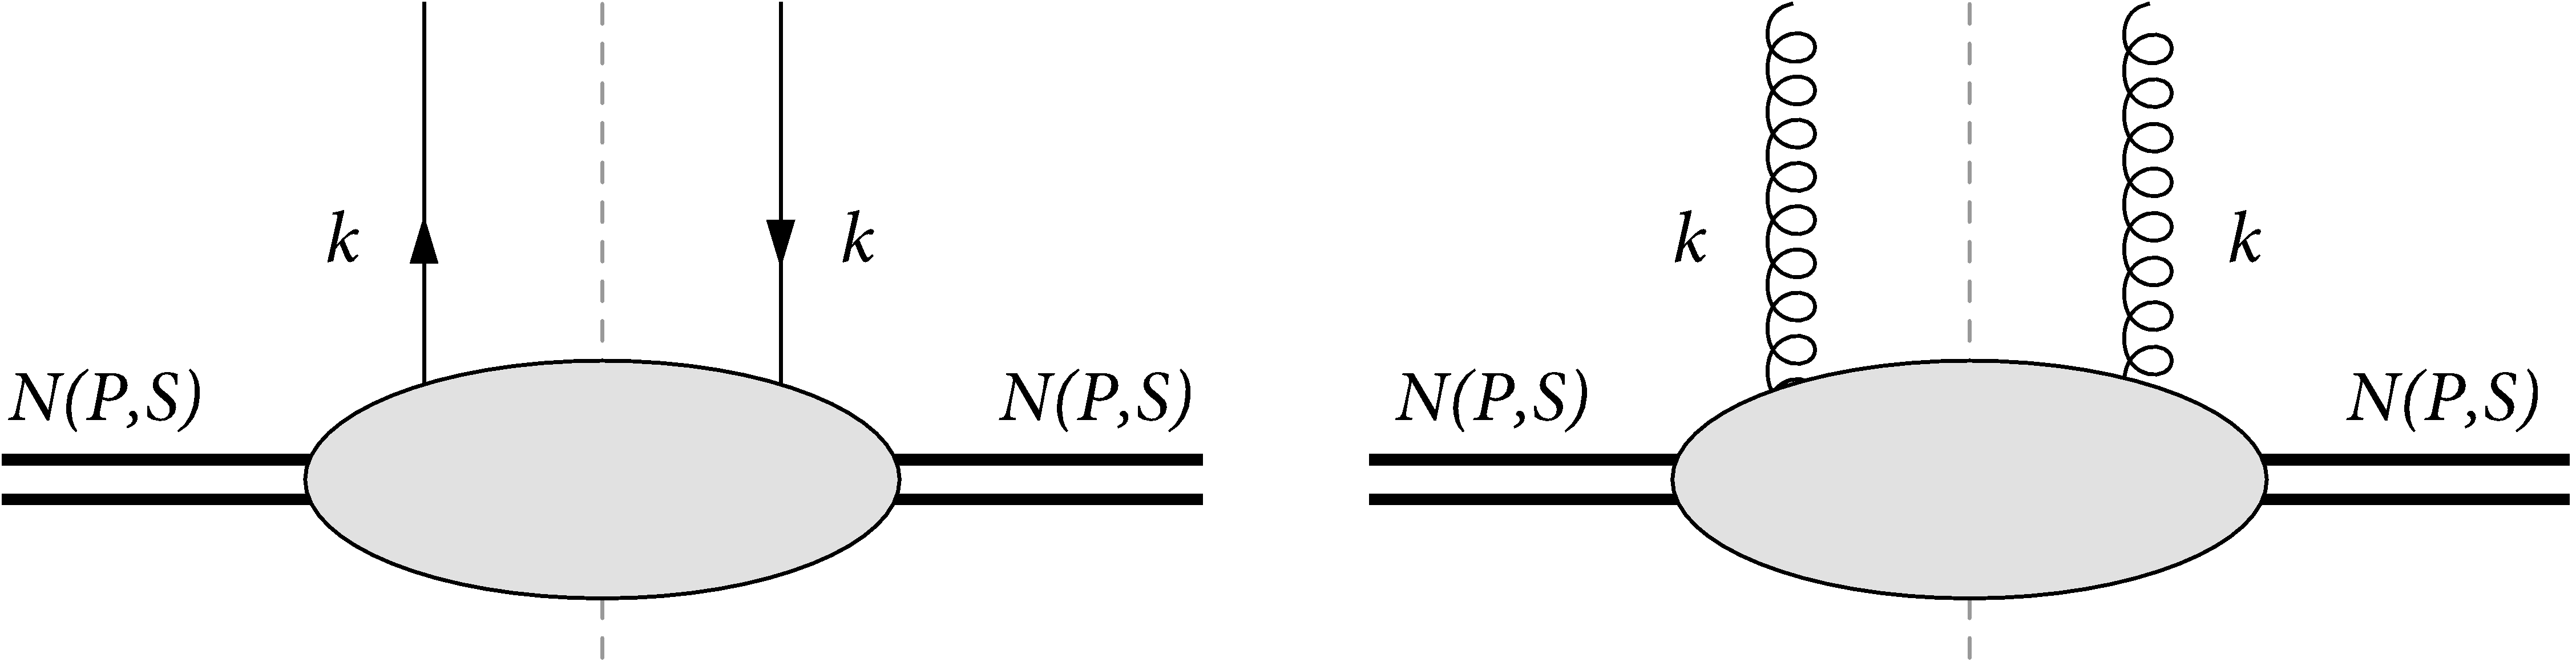
\includegraphics[width=0.8\linewidth]{fig/phi corr.png}
    \caption{Quark-quark (left) and gluon-gluon (right) distribution correlators appearing at leading-twist.}
    \label{fig:distribution corr}
\end{figure}

\subsection{Intrinsic twist-3 fragmentation}
The first type of sub-leading twist hadronic matrix elements are the so called \textit{intrinsic} twist-3 functions. They are expressed in terms of 2-parton correlations, involving a pair of quark fields or a pair of gluons. The fact that only one parton (on each side of the cut) is participating in the distribution/fragmentation process is a common feature with leading twist correlations.\\
Starting with the quark-quark case, these quantities are organized into a quark-quark fragmentation correlator
\begin{equation}
    \begin{aligned}
        \Delta^q_{ij}(z)&= \sum_X\int\frac{\dd \lambda}{2\pi} \,e^{-i\frac{\lambda}{z}}\mel{0}{\psi^q_i(0)}{h(P_h);X}\mel{h(P_h);X}{\bar \psi^q_j(\lambda m)}{0}\\
        &= \frac{1}{z}\left(\slashed{P}_h\right)_{ij} D^q_1(z)-\frac{iM_h}{2z} \left(\comm{\slashed{P}_h}{\slashed{m}}\right)_{ij} H^q(z)+\frac{M_h}{z}(\mathbb{1})_{ij}\,E^q(z)+\cdots,
        \end{aligned}
\end{equation}
where again the dots denote terms that are irrelevant for the present analysis. The $D_1(z)$ term is the familiar twist-2 unpolarized fragmentation function, appearing in numerous different high-energy processes involving the production of unpolarized hadrons. The sub-leading twist fragmentation function $H(z)$ describes the (power suppressed) production of unpolarized hadrons in the final state. The fact that twist-3 effects are generally smaller compared to the leading-twist case can be easily spotted by the fact they come with a mass factor $M_h$, the hadron mass. Compared to any hard scale, which we consider to be at least of the order of a some $\rm GeV$'s, typical produced hadron masses range from a few hunder $\rm MeV$'s ($\pi$) all they way up to a few $\rm GeV$'s ($\Lambda$). In this sense, the effect is said to be power suppressed.\\
One can also build a matrix element in which the exchanged parton coming from the nucleon is not a quark but rather a gluon. In this case, we only have leading twist effects, described in terms of a gluon-gluon fragmentation correlator CHECK
\begin{equation}
    \begin{aligned}
        \Delta^{g,\mu\nu}(z)&= \sum_X\int\frac{\dd \lambda}{2\pi} \,e^{-i\frac{\lambda}{z}} CHECK\\
        &= \frac{1}{z} g_T^{\mu\nu}\left(\slashed{P}_h\right)_{ij} D^g_1(z)+\cdots,
        \end{aligned}
\end{equation}
where $D_1^g(z)$ is the unpolarized gluon fragmentation function.

Similarly to distribution matrix elements, also fragmentation correlators are conveniently depicted as cut diagrams, as shown in Fig.~\ref{fig:fragmentation corr I}.
\begin{figure}[h]
    \centering
    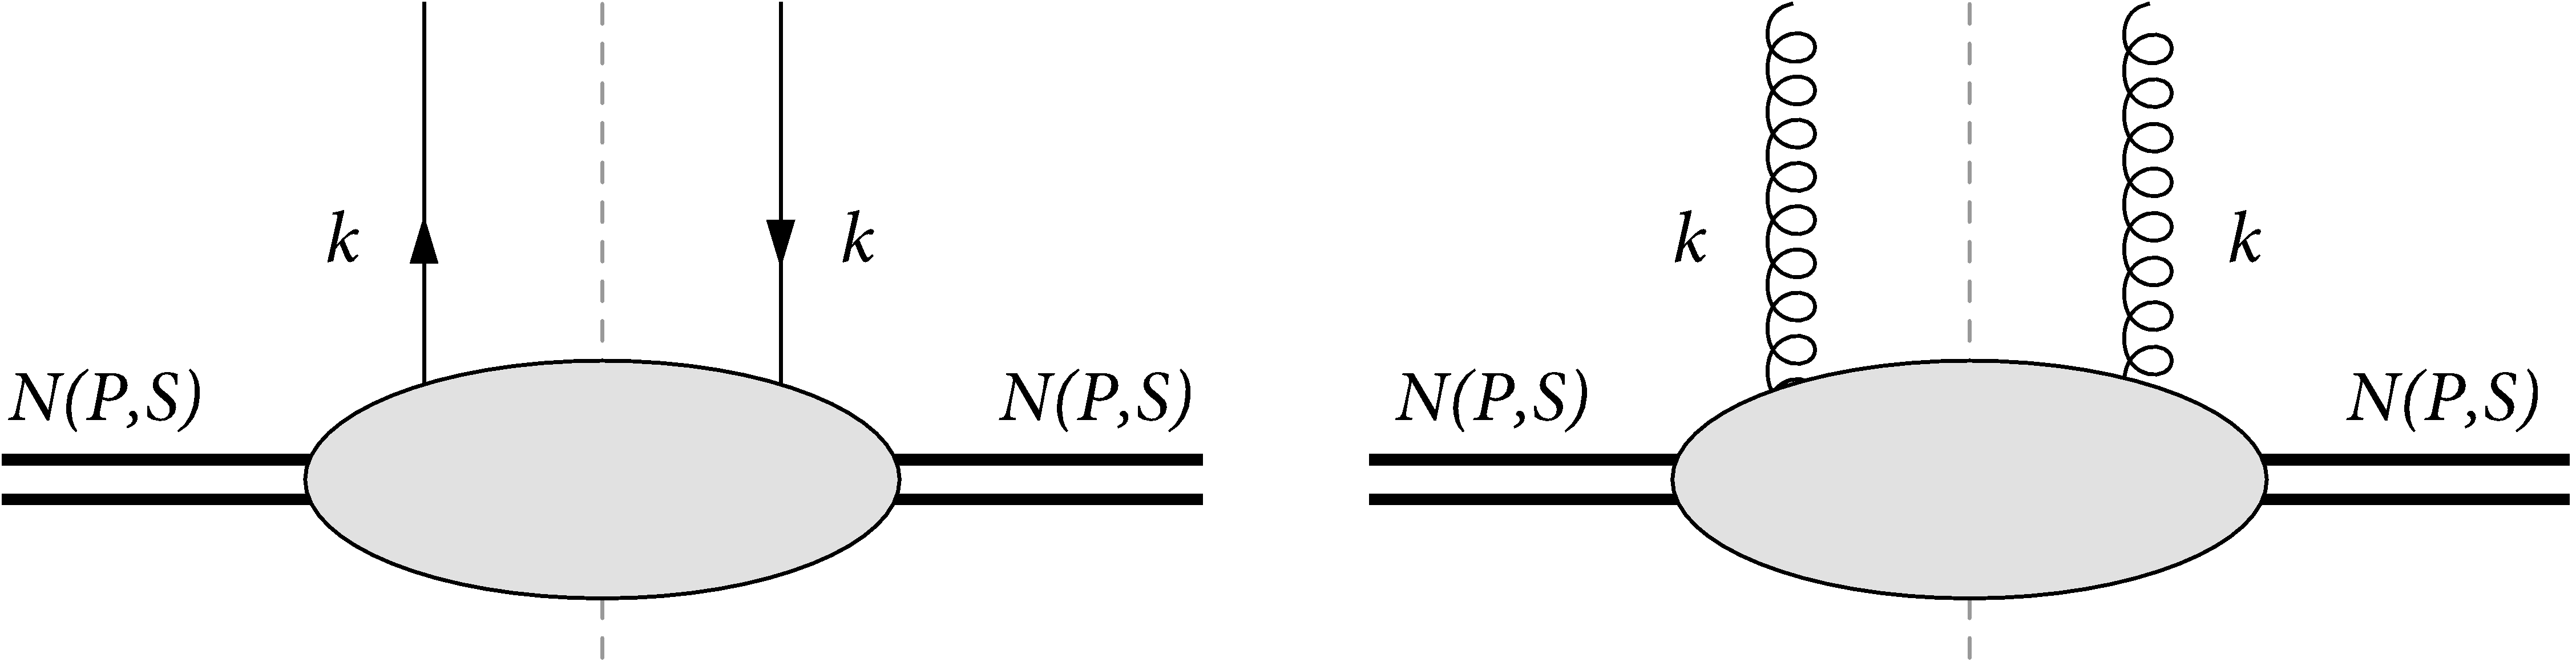
\includegraphics[width=0.8\linewidth]{fig/phi corr.png}
    \caption{Soft matrix elements relevant for leading twist and intrinsic twist-3 fragmentation. The quark-quark correlator (left) can depict both $D_1(z)$ or $H(z)$ depending on the Dirac structure assumed. The gluon-gluon correlator is also shown (right).}
    \label{fig:fragmentation corr I}
\end{figure}

\subsection{Kinematical twist-3 fragmentation}
Another kind of two-parton correlation functions are the so called \textit{kinematical} twist-3 functions. Contrary to the intrinsic twist-3 case, these objects incorporate (indirectly) also the transverse momentum dependence of partons. Instead of assuming the hadron and the fragmenting parton to be exactly collinear, now the kinematical approximation to the partonic momentum reads
\begin{equation}
    p^\mu = \frac{1}{z}P_h^\mu + p_T^\mu,
\end{equation}
where $p_T$ denotes the transverse partonic momentum. In practice, one performs a Taylor expansion to first order in $p_T$ in the hard scattering subprocess, commonly called the \textit{collinear expansion}. After this expansion, one often integrates out the transverse momentum, leaving us with a collinear matrix element. Keeping at first the full $p_T$-dependence into account, one may define a transverse momentum dependent (TMD) fragmentation correlator
\begin{equation}
    \begin{aligned}
        \Delta^q_{ij}(z,p_T)&= \sum_X\int\frac{\dd \lambda}{2\pi}\int\frac{\dd^{d-2}\eta_T}{(2\pi)^2} \,e^{-i\frac{\lambda}{z}-i\eta_T\cdot p_T}\\
        &\qquad\times\mel{0}{\psi^q_i(0)}{h(P_h);X}\mel{h(P_h);X}{\bar \psi^q_j(\lambda m+\eta_T)}{0}\\
        &= \frac{i z M_h}{2}\comm{\slashed{P}_h}{\slashed{m}}H^q(z,p_T)+\frac{iz}{2M_h}\comm{\slashed{p_T}}{\slashed{P}_h}H_1^{\perp,q}(z,p_T)\\
        &\quad +zM_h(\mathbb{1})_{ij}\,E^q(z,p_T)+\cdots  .
        \end{aligned}
\end{equation}
COMMENT ON FUNCTIONS\\
Now, the collinear matrix element relevant within the collinear twist-3 formalism is nothing else but the $p_T$-weighted correlator. It is
 \begin{equation}
    \begin{aligned}
        \Delta_{\partial,ij}^\rho(z)&= \int\dd^{d-2}p_T\,p_T^\rho\,\Delta_{ij}(z,p_T)\\
        &=\frac{z^{2\epsilon}}{z}\frac{i M_h}{2}\left(\comm{\slashed{P}_h}{\gamma^\rho}-\comm{\slashed{P}_h}{\slashed{m}}P_h^\rho\right)_{ij}H_1^{\perp(1)}(z)+ \cdots,
        \end{aligned}
\end{equation}
where the first moment of the Collins function is defined as the first $\vec{p_T}$ moment of the TMD fragmentation function CHECK Z!
\begin{equation}
    H_1^{\perp(1)}(z)=z^2\int \dd^2 p_T \frac{\vec{p_T}^2}{2 M_h^2}H_1^{\perp}(z,z^2 p_T^2).
\end{equation}

Kinematical twist-3 matrix elements are pictorially represented by the same kind of diagrams as the intrinsic twist-3 case. However, the kinematical approximation is different and one should keep in mind that the partonic momentum should have a transverse component, as shown in Fig.~\ref{fig:fragmentation corr K}

\begin{figure}[h]
    \centering
    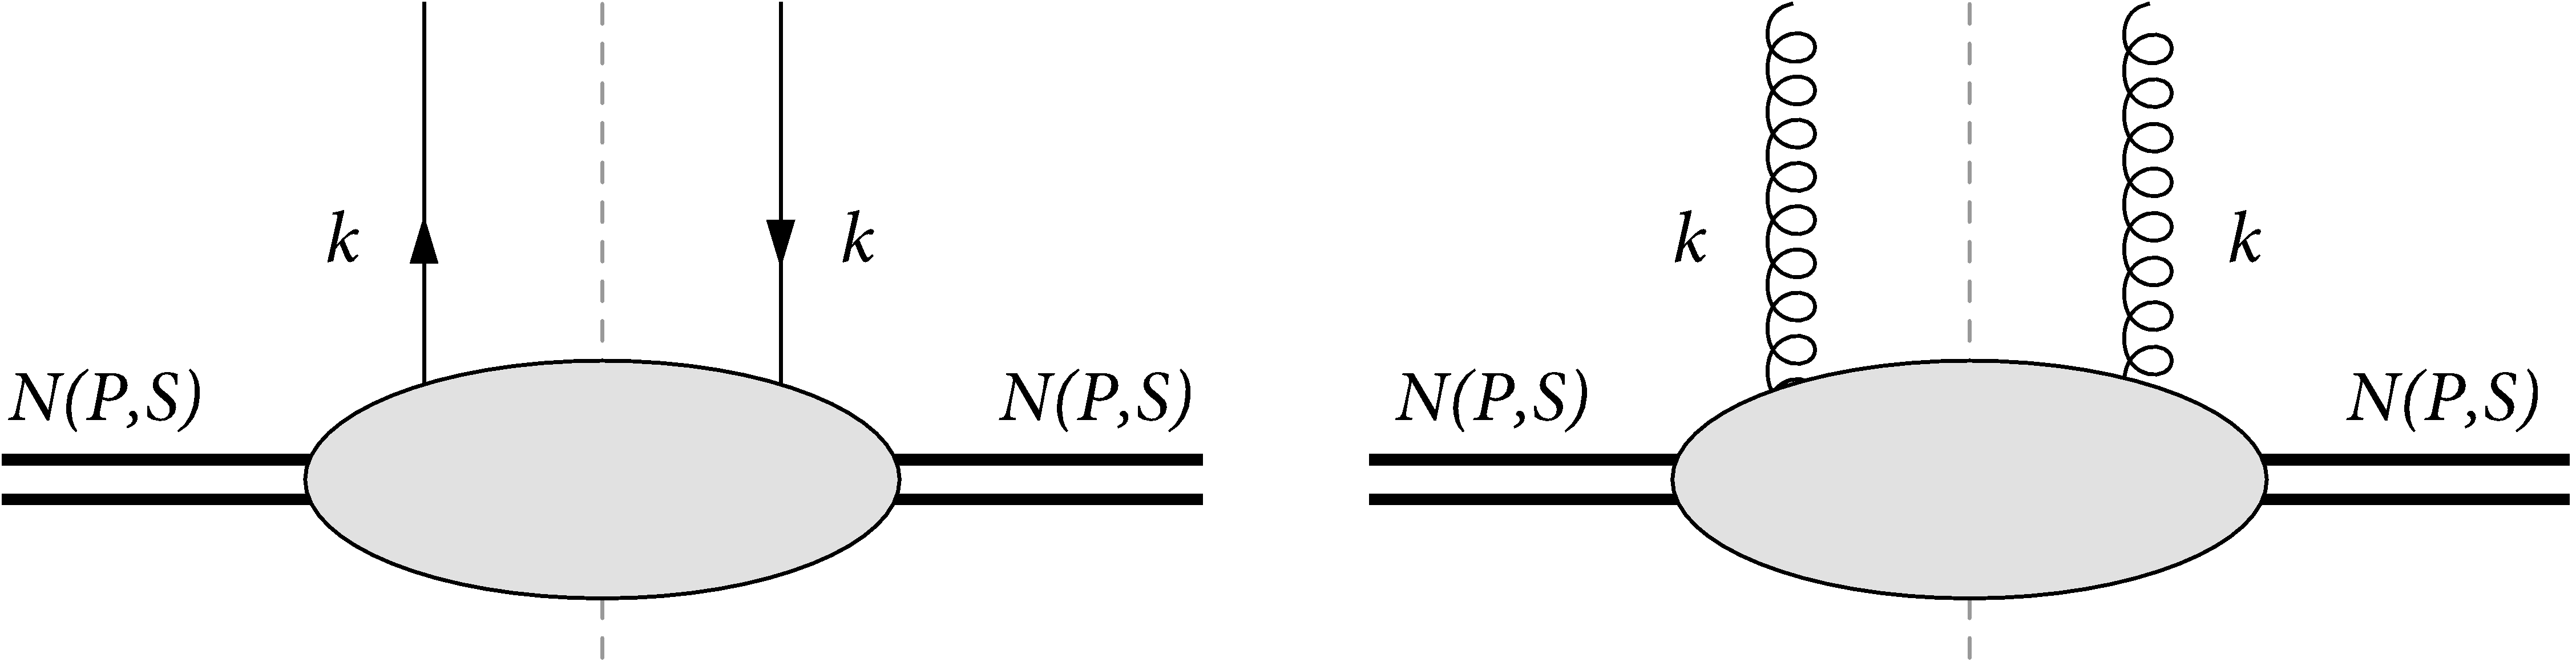
\includegraphics[width=0.8\linewidth]{fig/phi corr.png}
    \caption{Soft matrix element relevant for kinematical twist-3 fragmentation.}
    \label{fig:fragmentation corr K}
\end{figure}

\subsection{Dynamical twist-3 fragmentation}
The last type of twist-3 correlators are described in terms of matrix elements of three partonic fields, typically two quark/anti-quark fields and one gluonic field strength tensor. In general, such structures are composed of an interference of two transition amplitudes: one that is a coherent fragmentation of two partons into a hadron, and another that is the ordinary one-parton fragmentation. These objects are usually called \textit{dynamical} twist-3 correlation functions. Since the partons contributing to the hadron production are two, it makes sense that the matrix element will depend on more than one momentum fraction. The partonic momenta are now approximated as
\begin{equation}
    p^\mu = \frac{1}{z}P_h^\mu,\qquad p'^\mu = \frac{1}{z'}P_h^\mu.
\end{equation}
It is customary to introduce a scaled variable for the $z'$ momentum fraction, $z'= z/\zeta$, since it will simplify the treatment later on.

One type of dynamical twist-3 matrix elements are the so called \textit{quark-gluon-quark correlations}. In this case a quark and a gluon contribute to the final state hadronization process. The correlator is written as
%\begin{equation}
%    \begin{aligned}
%        \Phi^\rho_{F,ij}(x,x')&= \int\frac{\dd \lambda}{2\pi}\int\frac{\dd \eta}%{2\pi} \,e^{i\lambda x'+i\eta(x-x')}\mel{N(P,S)}{\bar \psi_j(0)\,i g_S\, %n_\sigma F^{\sigma \rho}(\eta n)\, \psi_i(\lambda n)}{N(P,S)}\\
%        &= \frac{M}{2}\epsilon^{Pn\rho S}\left(\slashed{P }\right)_{ij}\,i F_{FT}(x,%x')-\frac{M}{2}(S^\rho-(S \cdot n)P^\rho)\left(\slashed{P }\gamma_5\right)_%{ij}G_{FT}(x,x')+\cdots
%    \end{aligned}
%\end{equation}
\begin{equation}
    \begin{aligned}
        \Delta^{qg,\rho}_{F,ij}(z,\zeta)&= \sum_X\int\frac{\dd \lambda}{2\pi}\int\frac{\dd \eta}{2\pi} \,e^{-i\frac{\lambda }{z}\zeta-i\frac{\eta}{z}\left(1-\zeta\right)}\mel{0}{ig_S \mu^\epsilon m_\sigma F^{\sigma \rho}(\eta m)\psi_i(0)}{h(P_h);X}\\
        &\qquad \qquad \qquad \times\mel{h(P_h);X}{\bar \psi_j(\lambda m)}{0}\\
        &= z^{2\epsilon}\frac{iM_h}{2z}\left(\comm{\slashed{P}_h}{\gamma^\rho}-\comm{\slashed{P}_h}{\slashed{m}}P_h^\rho\right)_{ij}\,i\left(\hat H^{qg}_{FU}(z,z')\right)^*+\cdots,
        \end{aligned}
\end{equation}
where $\hat{H}_{FU}^{qg}$ is the quark-gluon-quark fragmentation function describing the production of unpolarized hadrons. 

Another kind of dynamical twist-3 matrix element is given by a quark-antiquark-gluon correlation. Intuitively, the fragmentation is initiated from a quark-antiquark pair. The relevant correlator is CHECK
\begin{equation}
    \begin{aligned}
        \Delta^{q \bar{q},\rho}_{F,ij}(z,\zeta)&= \sum_X\int\frac{\dd \lambda}{2\pi}\int\frac{\dd \eta}{2\pi} \,e^{-i\frac{\lambda }{z}\zeta-i\frac{\eta}{z}\left(1-\zeta\right)}CHECK\\
        &\qquad \qquad \qquad CHECK\\
        &= z^{2\epsilon}\frac{iM_h}{2z}\left(\comm{\slashed{P}_h}{\gamma^\rho}-\comm{\slashed{P}_h}{\slashed{m}}P_h^\rho\right)_{ij}\,i\left(\hat H^{q\bar{q}}_{FU}(z,z')\right)^*+\cdots,
        \end{aligned}
\end{equation}

ADD HERE BOUNDARY CONDITIONS AND SYMMETRIES ETC...\\

Lastly, the diagram notation for these dynamical twist-3 correlations is presented in Fig.~\ref{fig:fragmentation corr D}
\begin{figure}[h]
    \centering
    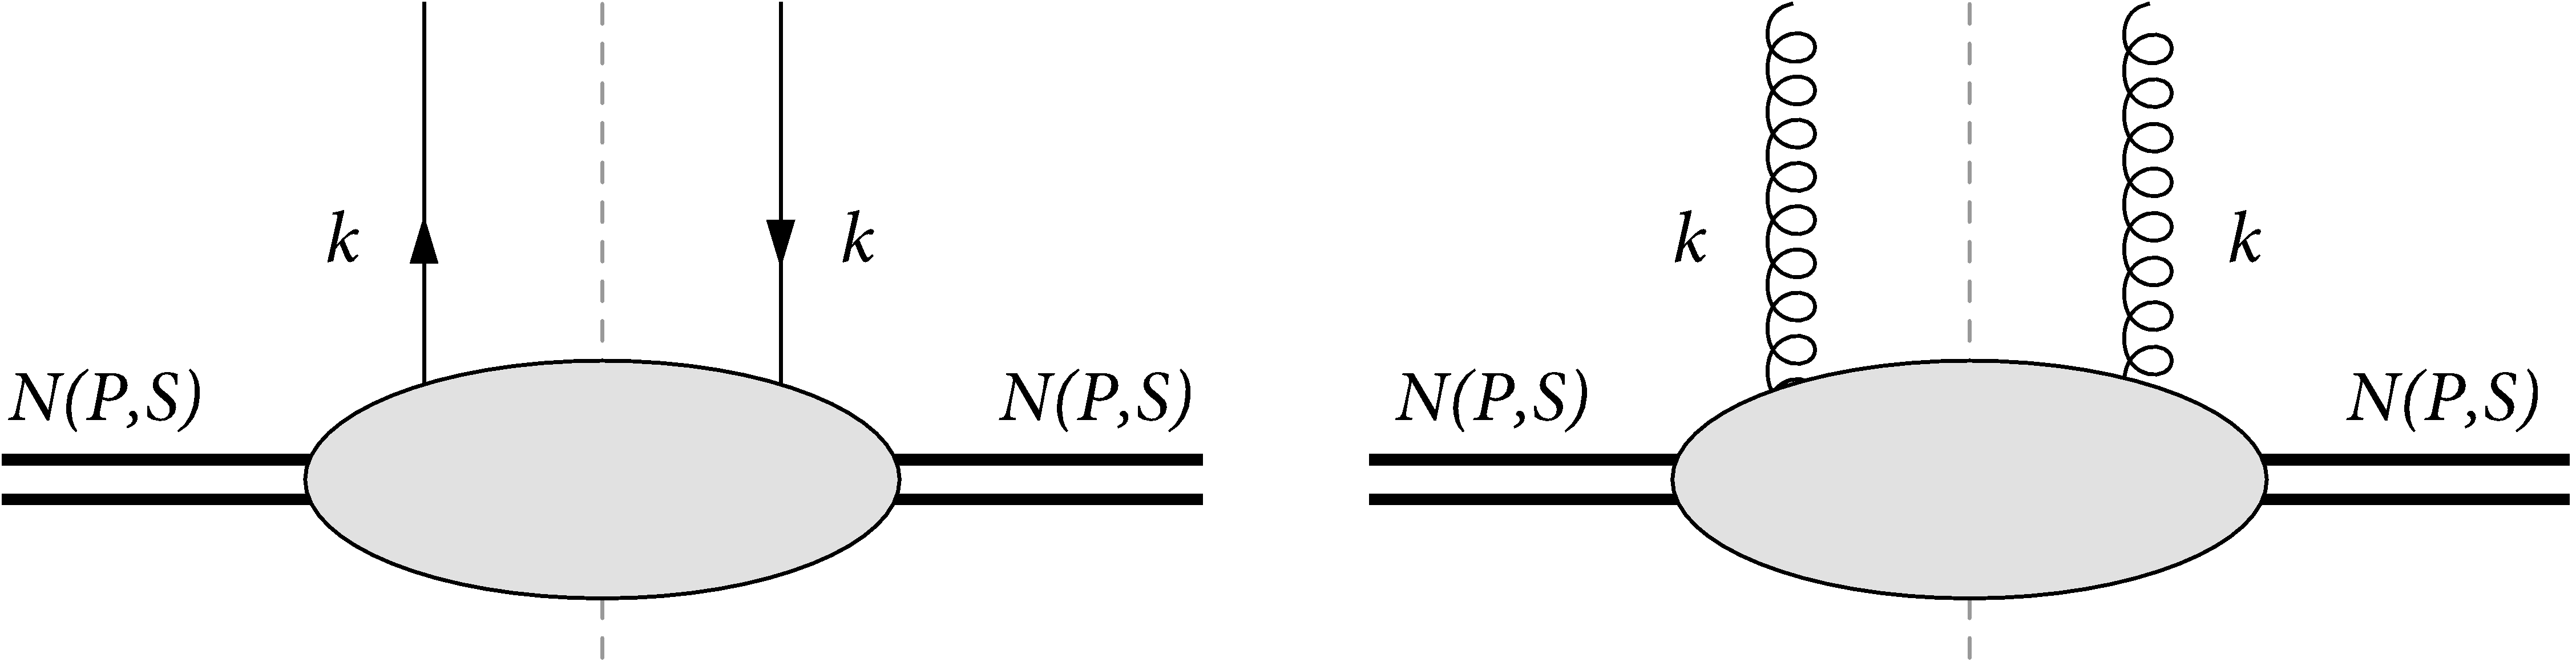
\includegraphics[width=0.8\linewidth]{fig/phi corr.png}
    \caption{Soft matrix element relevant for dynamical twist-3 fragmentation. Quark-gluon-quark (right) and quark-antiquark-gluon (left) correlations are shown.}
    \label{fig:fragmentation corr D}
\end{figure}



\section{QCD equation of motion relations}
\noindent ADD LITTLE DERIVATION OF EOM IN D DIMENSIONS! RELEVANT FOR THIS WORK!\\

The previously introduced twist-3 fragmentation functions are not independent from each other. In fact, they are related through the QCD equation of motion. The corresponding constraint equations will be referred as \textit{equation of motion relations} (EoMRs). These relations between sub-leading twist matrix elements can be derived by applying the QCD EOM to the relevant quark fields appearing in the correlators. The quark fields satisfy the equation
\begin{equation}
    \left(i \slashed{D}(x) -m_q \right)\psi^q(x)=0
\end{equation}
where $D_\mu^{ab}(x)=\delta^{ab}\partial_\mu -ig_S G_\mu^{ab}(x)$ is the usual covariant derivative in the fundamental representation. Decomposing the above equation on the light-cone and considering the matrix elements appearing in the various correlators \cite{bacchetta_semi-inclusive_2007}, one can derive the following relation \cite{kanazawa_operator_2016}
\begin{equation}\label{eq:eomr H}
    \frac{H^a(z)}{2 z}+H_1^{\perp(1)a}(z)= \mathcal{P}\int_0^1\dd \zeta\frac{\Im[\hat H^a_{FU}(z,z/\zeta)]}{1-\zeta}\qquad \text{(EoMR)}\,.
\end{equation}
Similar relations hold also for all the other twist-3 fragmentation functions, as well as for twist-3 parton distribution functions. Since other contributions do not enter our spin-dependent SIDIS cross section in the polarization case of interest, such EoMRs are irrelevant for the present work and we omit them here for brevity. At first glance, the above relation may seem redundant since it simply expresses the intrinsic and kinematical twist-3 fragmentation functions in terms of the dynamical one. However, as we will see in the next chapters, this relation is crucial to obtain a gauge invariant and infrared (IR) safe result for the final twist-3 cross section. In fact, when computing the hard scattering coefficients, one finds that they are not separately gauge invariant. Only after combining them according to the above EoMR, one obtains a gauge invariant result. This is a strong indication that the application of the QCD EoMR is not optional but it is rather an important and essential step in this kind of calculations.

\noindent ADD HERE GLUON EOMRs???\\

\noindent We also note in passing that one can find yet another fragmentation function in the literature, often denoted as $\tilde H(z)$. This functions is nothing else but a shorthand for a particular combination of $H$ and $H_1^{\perp(1)}$ or, equivalently, an (integrated) $\hat H_{FU}$ quark-gluon-quark correlation function. It is defined as
\begin{equation}\label{eq:Htildedefinition}
    \tilde{H}^a(z)=2z\,\mathcal{P}\int_0^1\dd \zeta\frac{\Im[\hat H^a_{FU}(z,z/\zeta)]}{1-\zeta}=H^a(z)+2z\,H_1^{\perp(1)a}(z).
\end{equation}
It is worth mentioning that this specific fragmentation function will play an important role in Chap.~\ref{chap:numerics}, when some numerical explorations of the $A_{UT}^{\sin\phi_S}$ asymmetry will be performed. In fact, for the first time, this collinear quark-gluon-quark function $\tilde{H}(z)$ has been extracted only recently from experimental data \cite{Gamberg2022Htilde}.



\section{Lorentz invariance relations}
Interestingly, there is yet another set of relations among twist-3 fragmentation functions, which are derived from the requirement of Lorentz invariance. These relations, called \textit{Lorentz invariance relations} (LIRs), can be obtained by considering the most general decomposition of the relevant correlators in terms of all possible Lorentz structures. By imposing that the correlators transform correctly under Lorentz transformations, one can derive constraints on the fragmentation functions and parton distribution functions. In particular, one finds that certain combinations of twist-3 fragmentation functions must vanish. For our purposes, the most relevant LIR is \cite{kanazawa_operator_2016}
\begin{equation}
    \frac{H^a(z)}{z}=-\left(1-z\frac{\dd}{\dd z}\right)H_1^{\perp(1)a}(z)-2\int_0^1 \dd \zeta\frac{\Im[\hat H^a_{FU}(z,z/\zeta)]}{\left(1-\zeta\right)^2}\qquad \text{(LIR)}\,.
\end{equation}
Very similarly to the EoMR case, this relation can be essential to obtain a Lorentz invariant twist-3 cross section. In fact, a priori, twist-3 cross sections may be frame dependent, since the partonic coefficients depend on the light-cone vectors $n^\mu$ and $m^\mu$, which in turn depend on the choice of reference frame. As clearly seen in the previous paragraphs, the parametrization of twist-3 matrix elements depends explicitly on these vectors. The fact that twist-3 observables explicitly involve these light-cone vectors is intuitively clear. This is because any twist-3 observable is sensitive to the transverse component of some vector (e.g. the transverse spin component, etc...) and in order to define what "transverse" means one needs to introduce two light-cone vectors. As one sees, it is only after applying LIRs that one obtains a frame independent result and sees the manifest Lorentz invariance of the cross section. 
